\section{Overview of the pseudonymization procedure}
\label{section:overview}
ALIIAS has a number of assumption about the underlying experimental procedures. These assumptions were defined so that they are easy to fit to the majority of medical research experiments. The pseudonymization workflow of SFB289 is illustrated on Fig. \ref{fig:flowchart} and includes the following steps.

\begin{figure}[H]
\centering
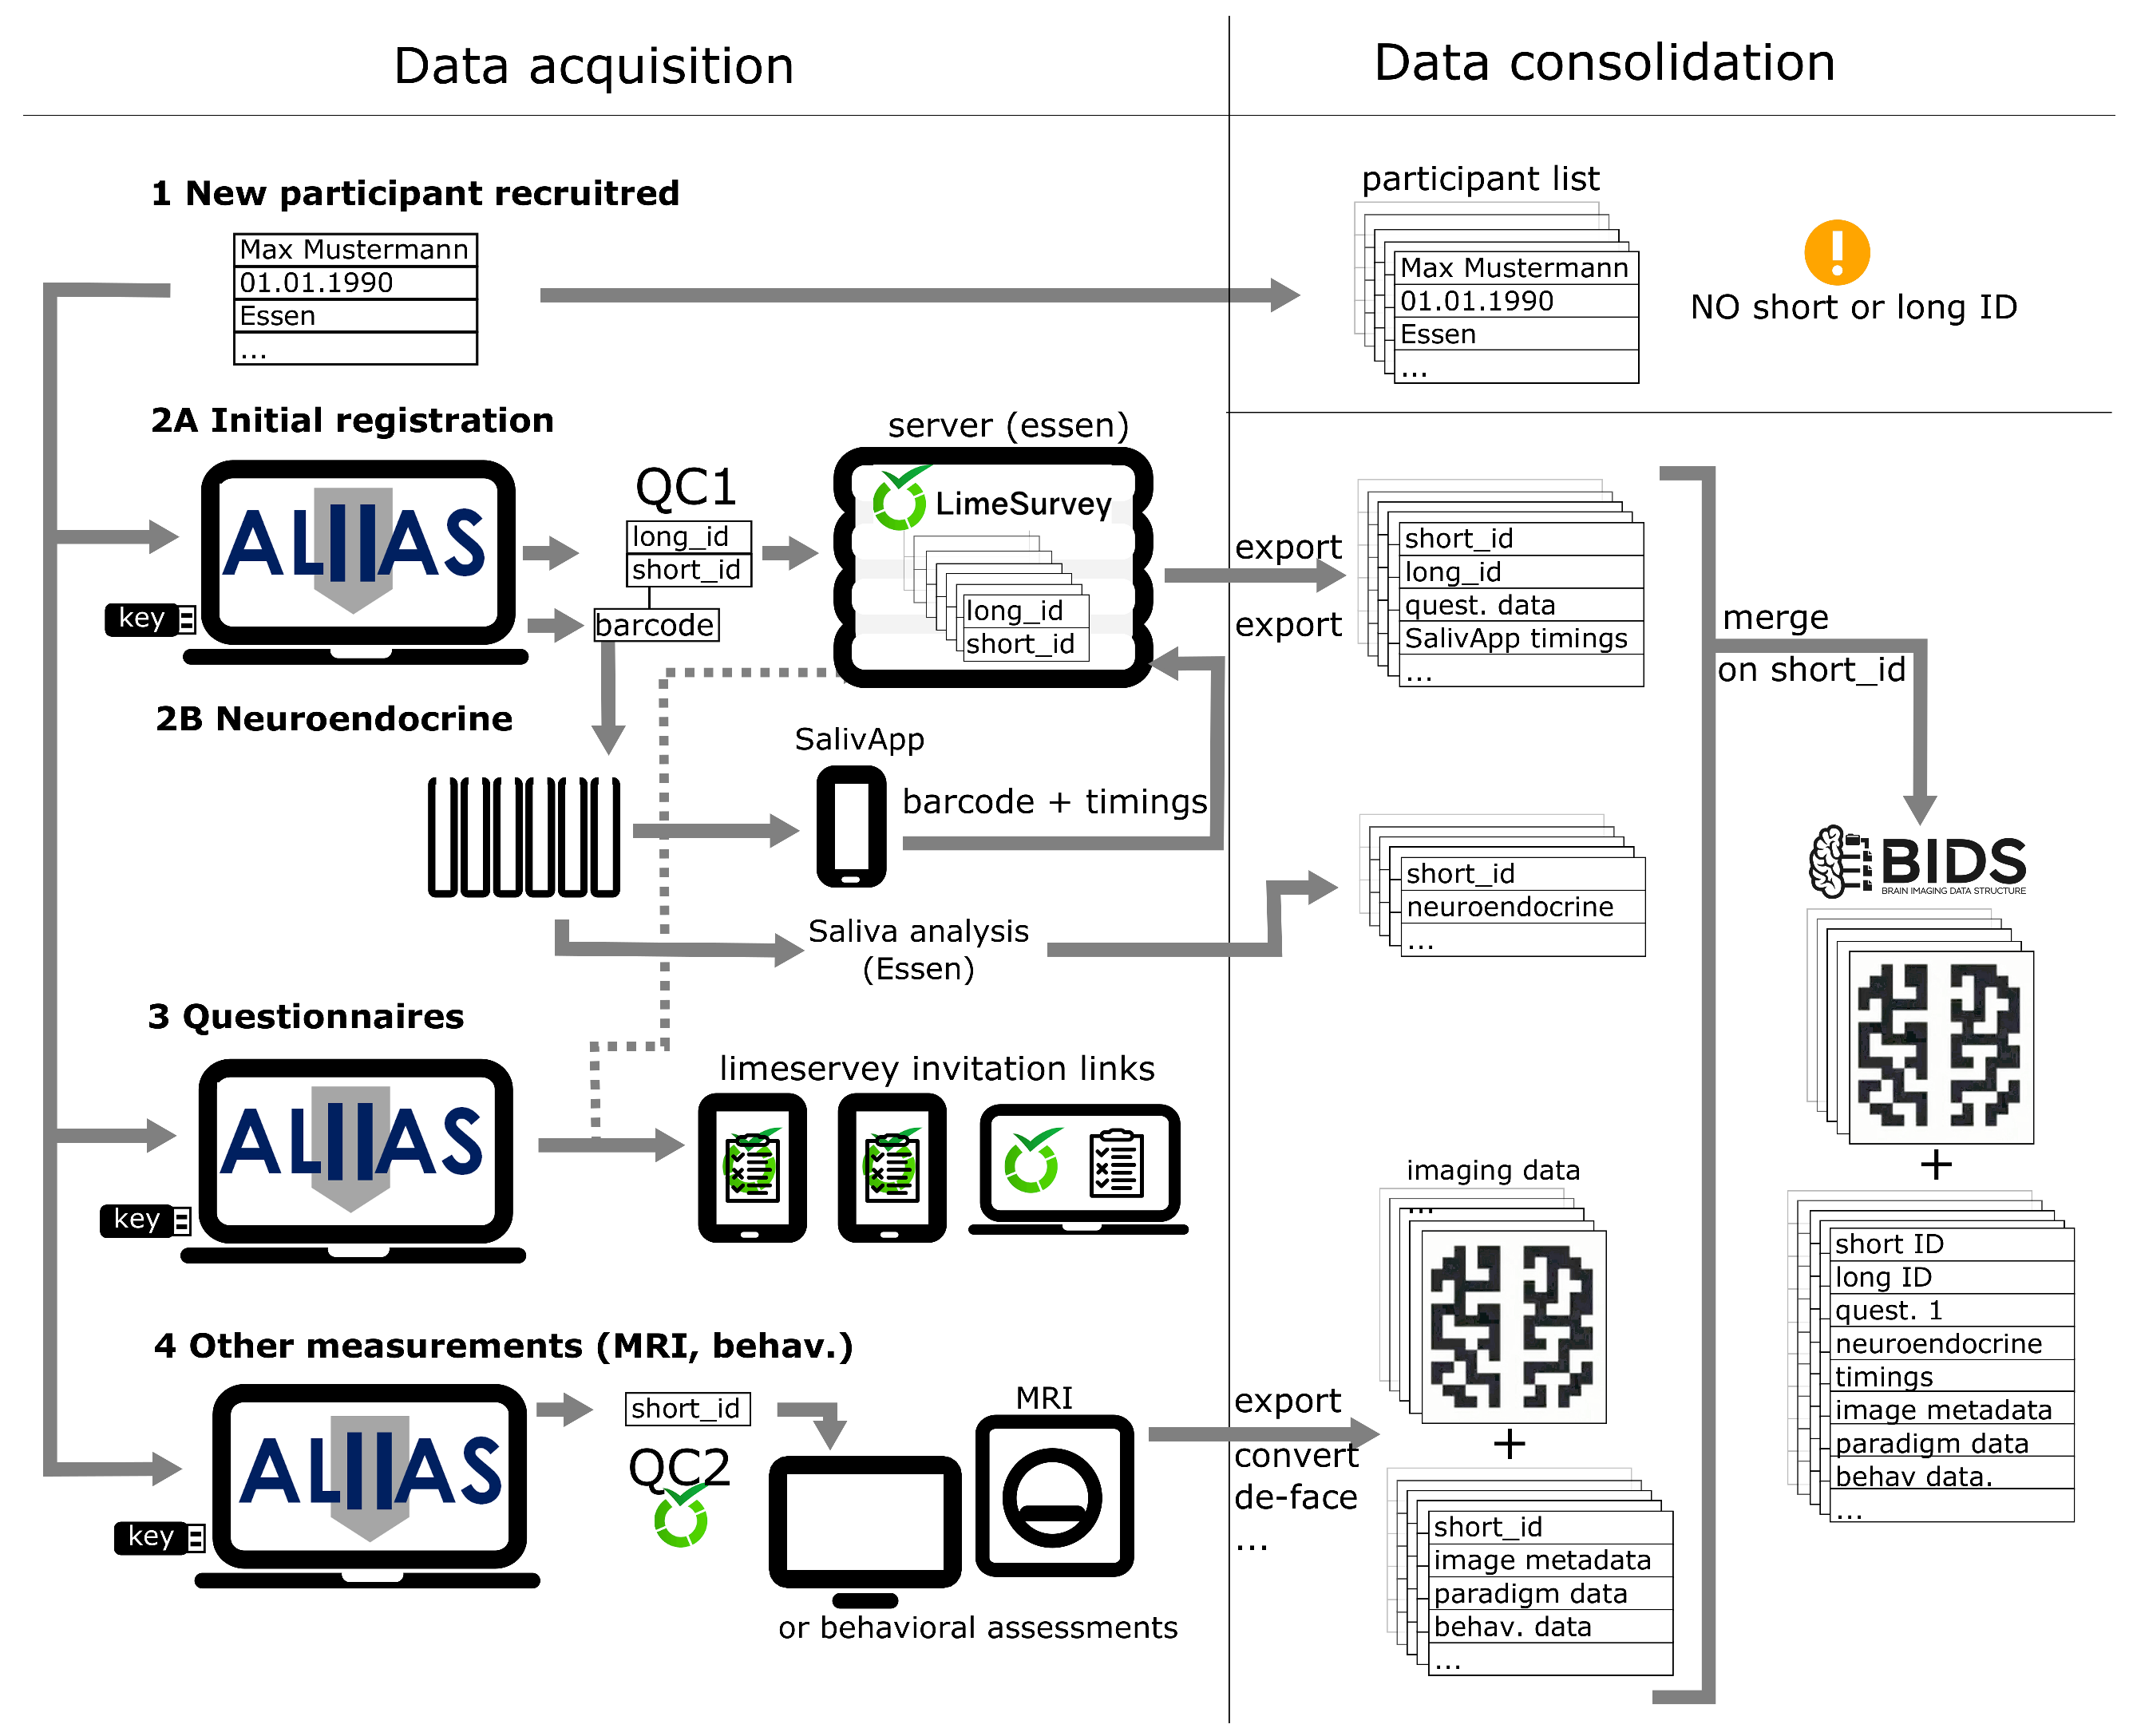
\includegraphics[width=1.0\textwidth]{docs/fig/overview_v3.eps}
\caption{The pseudonymization workflow of SFB289}
\label{fig:flowchart}
\end{figure}

\InsertBoxR{1}{
\small\setlength\fboxsep{5pt}\setlength\fboxrule{1pt}
\fcolorbox{pniblue}{pniblue!5}{\begin{minipage}{0.5\textwidth}
Important Note: the pseudonyms must never be stored in the participant list!
\end{minipage}}
}[1]

\par\noindent\rule{\textwidth\color{pniblue}}{0.4pt}
\textbf{1. Participant recruitment:}
\addcontentsline{toc}{subsubsection}{Participant recruitment}
When a new participant is recruited, his/her personal data and contact details (e.g. address, phone number, e-mail) is recorded on-site (or e.g. during a telephone interview). These data is typically saved into a "participant list" (often an excel table, its maintenance is the responsibility of the single projects, see Fig. \ref{fig:flowchart}). While this participant list itself is also to be protected, ALIIAS is not reliable for the protection of this data. In fact, the main goal of ALIIAS is to make it impossible to link this data to the experimental datasets (unless owning the pseudonymization secret, i.e. the hardware key).
%%\par\noindent\rule{\textwidth\color{pniblue}}{0.4pt}
%\InsertBoxR{-1}{
%\small\setlength\fboxsep{5pt}\setlength\fboxrule{1pt}
%\fcolorbox{pniblue}{pniblue!5}{\begin{minipage}{0.45\textwidth}
%Importantly, even though the web browser is used as a user interface for the software %(thus it looks like a webpage), personal data always stays on the local computer hosting %the software and hardware key.
%\end{minipage}}
%}[1]


\par\noindent\rule{\textwidth\color{pniblue}}{0.4pt}
\addcontentsline{toc}{subsubsection}{Initial registration}
\textbf{2A. Initial registration:} The dedicated hardware key (provided by Z03) is connected to an experimental computer (with ALIIAS already installed) via the USB port. As a next step, the researcher enters the LimeSurvey login credentials in ALIIAS and the provides the following personal data of the participant on the browser interface of ALIIAS (depicted on the left of Fig. \ref{fig:screenshots}):
\begin{itemize}
    \item first name
    \item last name
    \item date of birth
    \item place of birth
    \item mother's maiden name
\end{itemize}

Importantly, even though the web browser is used as a user interface for the software (thus it looks like a webpage), \textbf{personal data always stays on the local computer}, which hosts the software and hardware key.


\begin{figure}[H]
%\centering
\subfigure{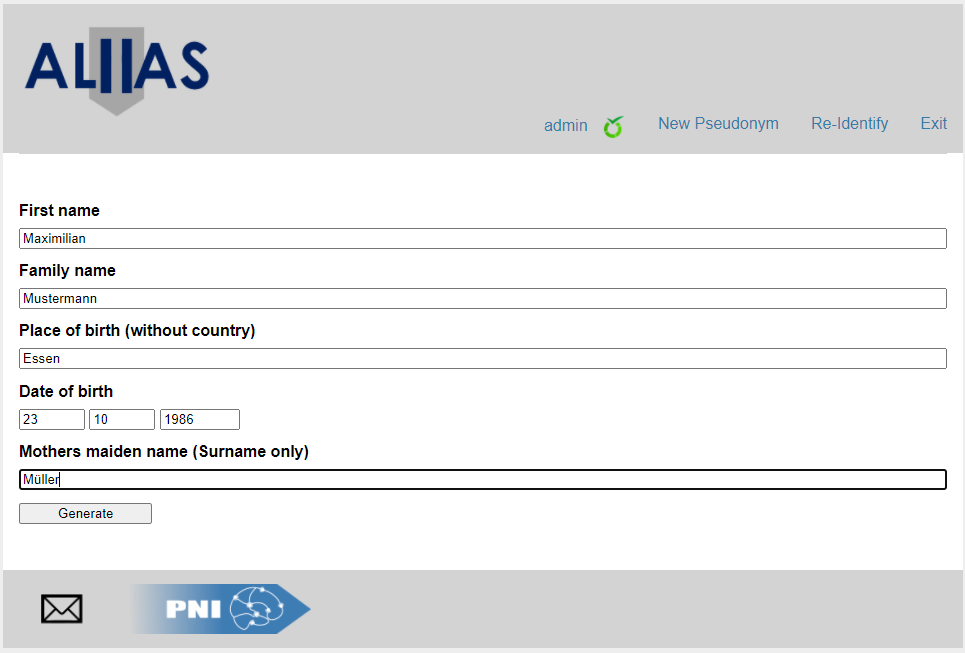
\includegraphics[width=.45\textwidth]{docs/fig/03_filled.PNG}}
\hfill
\subfigure{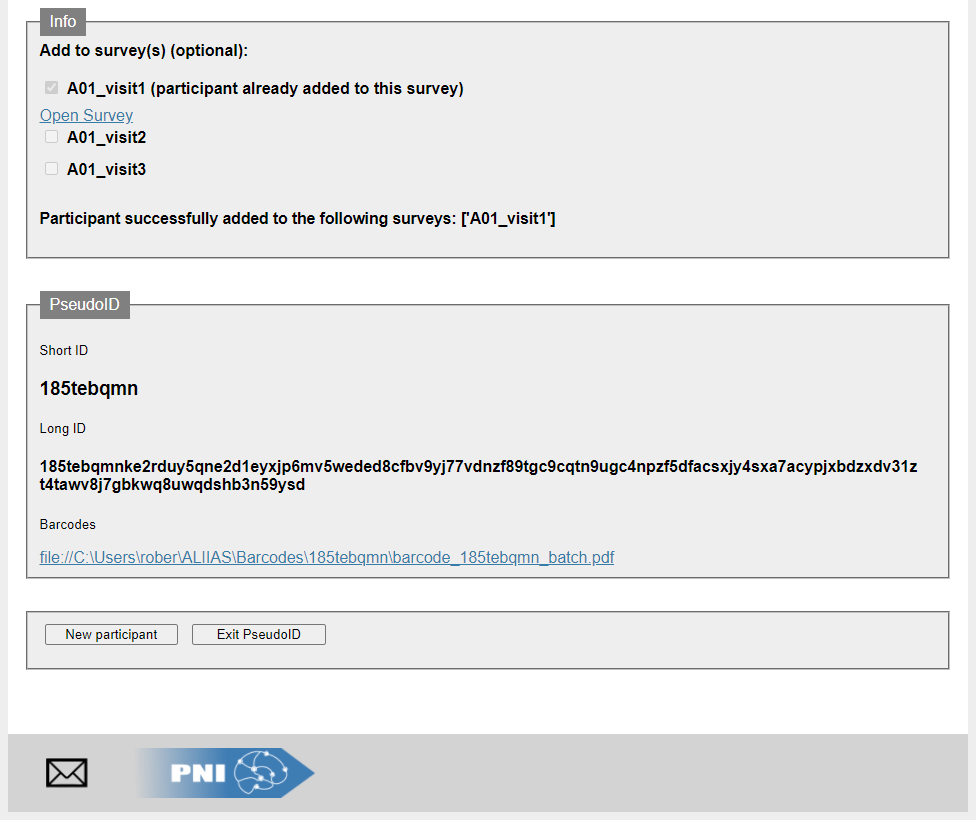
\includegraphics[width=.45\textwidth]{docs/fig/05_pseudonym.PNG}}
\caption{The browser-based user interface of ALIIAS.}
\label{fig:screenshots}
\end{figure}

ALIIAS reads the "pseudonymization secret" from the hardware key and uses it to generate pseudonym. After the user confirms that the data is correct, the software outputs the long and short-version of the pseudonym (on the right of Fig. \ref{fig:screenshots}). Both the long and short IDs are unique for the whole CRC. De-identification is only possible with the long-id. During the initial registration, ALIIAS automatically connects to the LimeSurvey server hosted at the University Duisburg-Essen and registers the participant's long and short IDs to any of the surveys belonging to the single project. Additionally, ALIIAS converts the short ID into a barcode (see step 5) for labelling assessment tools belonging to the participant.

\par\noindent\rule{\textwidth\color{pniblue}}{0.4pt} 
\addcontentsline{toc}{subsubsection}{Compatibility with neuroendocrine and genetic assessments}
\textbf{2B. Compatibility with neuroendocrine and genetic assessment and Biobank:} Upon the initial registration, ALIIAS generates a set of barcodes, encoding the short ID. These will be printed by the barcode printers provided by the central projects and used to label the saliva sampling kit (+ genetics) for the given participant (refer to the corresponding SOP of Z02). These barcode labels will be scanned by the participant, using the dedicated smartphone application of SFB289 (SalivApp), directly after during sample collection (for precise timing). The ShortID encoded in the barcode is obtained in Z02 to link saliva sample results with sample timings, genetics and BioBank-IDs.

\par\noindent\rule{\textwidth\color{pniblue}}{0.4pt}
\addcontentsline{toc}{subsubsection}{Questionnaires}
\textbf{3. Questionnaires:}
 In SFB289, questionnaire data will be collected with LimeSurvey. After the participant has been assigned to a survey, ALIIAS provides an individualized invitation link, which can be opened in another browser tab or e-mailed to the participant. Questionnaires can be filled in on any computer (or tablet), with internet connection. 
 If the initial registration and the assignment of the participant to a given questionnaire take place in different time points (e.g repeated measures), ALIIAS can be used again and again to obtain the (permanent) short ID of the participant, given his/her personal data (either from the local 'participant list', see step 1., or as provided by the participant.
 Multiple assessment points (repeated measures) are handled as separate surveys in LimeSurvey (refer to section \ref{section:ls_setup} for more details).
 
 \par\noindent\rule{\textwidth\color{pniblue}}{0.4pt}
 \addcontentsline{toc}{subsubsection}{Other measurements}
 \textbf{4. Other measurements (MRI, behavior):}
 For other measurements, ALIIAS can be used repeatedly to obtain the shortID of the participant (given the hardware key). The short ID can than be used in the dedicated experimental system (e.g. the MRI console) as the identifier ("name") of the participant, so that it gets exported together with the experimental data. In case of repeated measurements, ALIIAS is simply used multiple times to obtain the short ID. Single projects can add arbitrary "experimental tags" to the short ID (e.g. append '-w2' for week 2) or use the built in features of the given experimental equipment (e.g. separate 'program cards' on the MRI console) to distinguish between measurements.

\par\noindent\rule{\textwidth\color{pniblue}}{0.4pt}
\addcontentsline{toc}{subsubsection}{Data Consolidation and re-identification}
\textbf{Data Consolidation and re-identification:} The experimental data (either exported form the LimeSurvey database, or via the dedicated experimental systems) - if required - will be subject of further anonymization (e.g. de-facing of structural MRI images) The central scientific project will provide recommendations and share software tools for these tasks. Merging of experimental data from different sources or different assessment points is based on the short ID. The LimeSurvey database provides the link between the short and long IDs. The latter can be used for re-identification, e.g. in case of incidental findings by the owners of the hardware key.